%!TEX root = ../main.tex
\newcommand{\body}{\ensuremath{\t{body}}\xspace}
\newcommand{\strokewidth}{\ensuremath{\t{stroke\_w}}\xspace}
\newcommand{\segmentationpoints}{\ensuremath{\t{sps}}\xspace}
\newcommand{\segmentationpoint}{\ensuremath{\t{sp}}\xspace}
\newcommand{\image}{\ensuremath{\t{image}}\xspace}
\newcommand{\subimage}{\ensuremath{\t{sub\_image}}\xspace}
\newcommand{\leftsubimage}{\ensuremath{\t{left}}\xspace}
\newcommand{\rightsubimage}{\ensuremath{\t{right}}\xspace}
\newcommand{\segmentfurther}{\ensuremath{\t{todo}}\xspace}
\newcommand{\characters}{\ensuremath{\t{done}}\xspace}
\newcommand{\parameters}{\ensuremath{\t{parameters}}\xspace}

\begin{figure}
	%!TEX root = ../main.tex
\MakeRobust{\Call}

\newcommand{\body}{\ensuremath{\mathit{body}}\xspace}
\newcommand{\strokewidth}{\ensuremath{\mathit{stroke\_w}}\xspace}
\newcommand{\segmentationpoints}{\ensuremath{\mathit{sps}}\xspace}
\newcommand{\segmentationpoint}{\ensuremath{\mathit{sp}}\xspace}
\newcommand{\image}{\ensuremath{\mathit{image}}\xspace}
\newcommand{\subimage}{\ensuremath{\mathit{sub\_image}}\xspace}
\newcommand{\leftsubimage}{\ensuremath{\mathit{left}}\xspace}
\newcommand{\rightsubimage}{\ensuremath{\mathit{right}}\xspace}
\newcommand{\segmentfurther}{\ensuremath{\mathit{todo}}\xspace}
\newcommand{\characters}{\ensuremath{\mathit{done}}\xspace}
\newcommand{\parameters}{\ensuremath{\mathit{parameters}}\xspace}

\begin{algorithmic}[1]
\Function{segment}{$\image,\, \parameters$}
\State \body $\gets$ \Call{body\_region}{\image}
\State \strokewidth $\gets$ \Call{stroke\_width}{\image} 
\item[]
\State \segmentationpoints $\gets$ \Call{segmentation\_points}{\body, \strokewidth} 
\State \segmentfurther \characters $\gets$ [\image], []
\item[]
\While{\Call{continue}{~}}
	\State $\subimage \gets$ \Call{select\_sub\_image}{\segmentfurther} 
	\State $\segmentationpoint \gets$ \Call{select\_sp}{\segmentationpoints} 
	\State \leftsubimage, \rightsubimage $\gets$ \Call{split}{\subimage, \segmentationpoint}
	%
   \If {\Call{is\_character}{\leftsubimage}}
      \State \Call{add}{\leftsubimage, \characters}
   \Else
		\State \Call{add}{\leftsubimage, \segmentfurther}
   \EndIf \Comment{Repeat for \rightsubimage.}
\EndWhile
\State \textbf{return} \Call{merge}{\segmentfurther, \characters}
\EndFunction
\end{algorithmic}
	\caption{Binary Over Segmentation Algorithm.}
	\label{alg:method:segmentation:algorithm}
\end{figure}

We use binary over segmentation to segment the words into images, the pseudo code of this algorithm is presented in \cref{alg:method:segmentation:algorithm}. This algorithm aims to segment an image into two sub-images on the segmentation point that is most likely. One of these sub images is then selected and segmented again into two new sub-images, if it is not a character. This is repeated until the termination condition has been reached, i.e. \function{continue}{} is not longer true. If the segmentation has finished the list with images that could be segmented further, \segmentfurther, and the list with characters, \characters, are merged by \function{merge}. This function ensures that the final returned list of character images is in the same order as the characters occur in the word image. \Cref{fig:method:segmentation:tree} illustrates how the algorithm segments an images of a word into images of characters.

The \parameters passed to \function{segment}{} in \cref{alg:method:segmentation:algorithm} contain the maximum character length and the minimum, average and maximum image width and height. The maximum word length is the length of the longest word in the data set. The other six values are determined based on the data. Before computing the minimum, average or maximum all widths, or heights, that are not within two standard deviations of the mean of the character widths, or heights, are discarded as outliers. 

The different functions referenced in \cref{alg:method:segmentation:algorithm} are discussed in \crefrange{sss:method:segmentaton:bodyregion}{sss:method:segmentaton:termination}.

\begin{figure}
	\centering
	\timemachine{Create this image, as a tree with the word image as the root and the character image as the leaf. In the images mark the used segmentation line. Don't show left over segmentation lines in the leaves.}
	\missingfigure{Visualize how a word is segmented, using a tree view. Sort of like \cref{fig:introduction:binaryOversegmentation:chainfailure}.}
	\caption{Caption here}
	\label{fig:method:segmentation:tree}
\end{figure}

\subsubsection{Body Region}
\label{sss:method:segmentaton:bodyregion}
	The body region is the part of the image that is between the lower and the upper base line. To compute the low base line for each column in the image the lowest row with a foreground pixel is computed. The low base line is the mode of the these rows. The high baseline is computed in the same way, but uses the highest row of each column with a foreground pixel. 

	The part of the image between the low and high base line is the body region. Using this region for the computation of the segmentation points reduces the influence of extensive ligatures. \Cref{fig:method:segmentation:baseline} illustrates examples of the determination of the baselines. \Cref{fig:method:segmentation:baseline:succes} reflects the intended outcome, the second example, \cref{fig:method:segmentation:baseline:failure}, draws the upper baseline too high because of the extra curve on the last letter.

	\begin{figure}
		\centering
		\subfloat[]{
			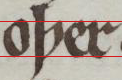
\includegraphics[height=7em]{shared/img/method/base_line_succes.png}%
			\label{fig:method:segmentation:baseline:succes}%
		}
		\hspace{0.05\columnwidth}
		\subfloat[]{
			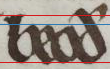
\includegraphics[height=7em]{shared/img/method/base_line_fail.png}%
			\label{fig:method:segmentation:baseline:failure}%
		}
		\caption{An example of \protect\subref{fig:method:segmentation:baseline:succes} correct and \protect\subref{fig:method:segmentation:baseline:failure} incorrect baselines found with the described method. The found baselines are shown in red. If the found baselines were incorrect, the correct baselines are shown in blue.}
		\label{fig:method:segmentation:baseline}
	\end{figure}

\subsubsection{Stroke Width}
\label{sss:method:segmentaton:strokwidth}
	The stroke width refers to how thick the stroke of a pen is. We compute the stroke width as the mode of the number of sequential foreground pixels in one row or column of pixels in the horizontal and the vertical direction respectively. The stroke width is computed per image instead of per page or data set word to be able to handle text written by different authors or with different pens on the same page.

\subsubsection{Segmentation Points}
\label{sss:method:segmentaton:segmentationpoints}
	To find the segmentation lines we first determine the suspicious regions. A suspicious region is a region in the body of the word image where the vertical pixel density is greater than some threshold, we have set this threshold to $2 \cdot \strokewidth$, \cref{fig:method:segmentation:suspiciousRegions} illustrates the suspicious regions found in a word. 

	\begin{figure}
		\timemachine{Create this image based on our dataset ourselves.}
		\centering
		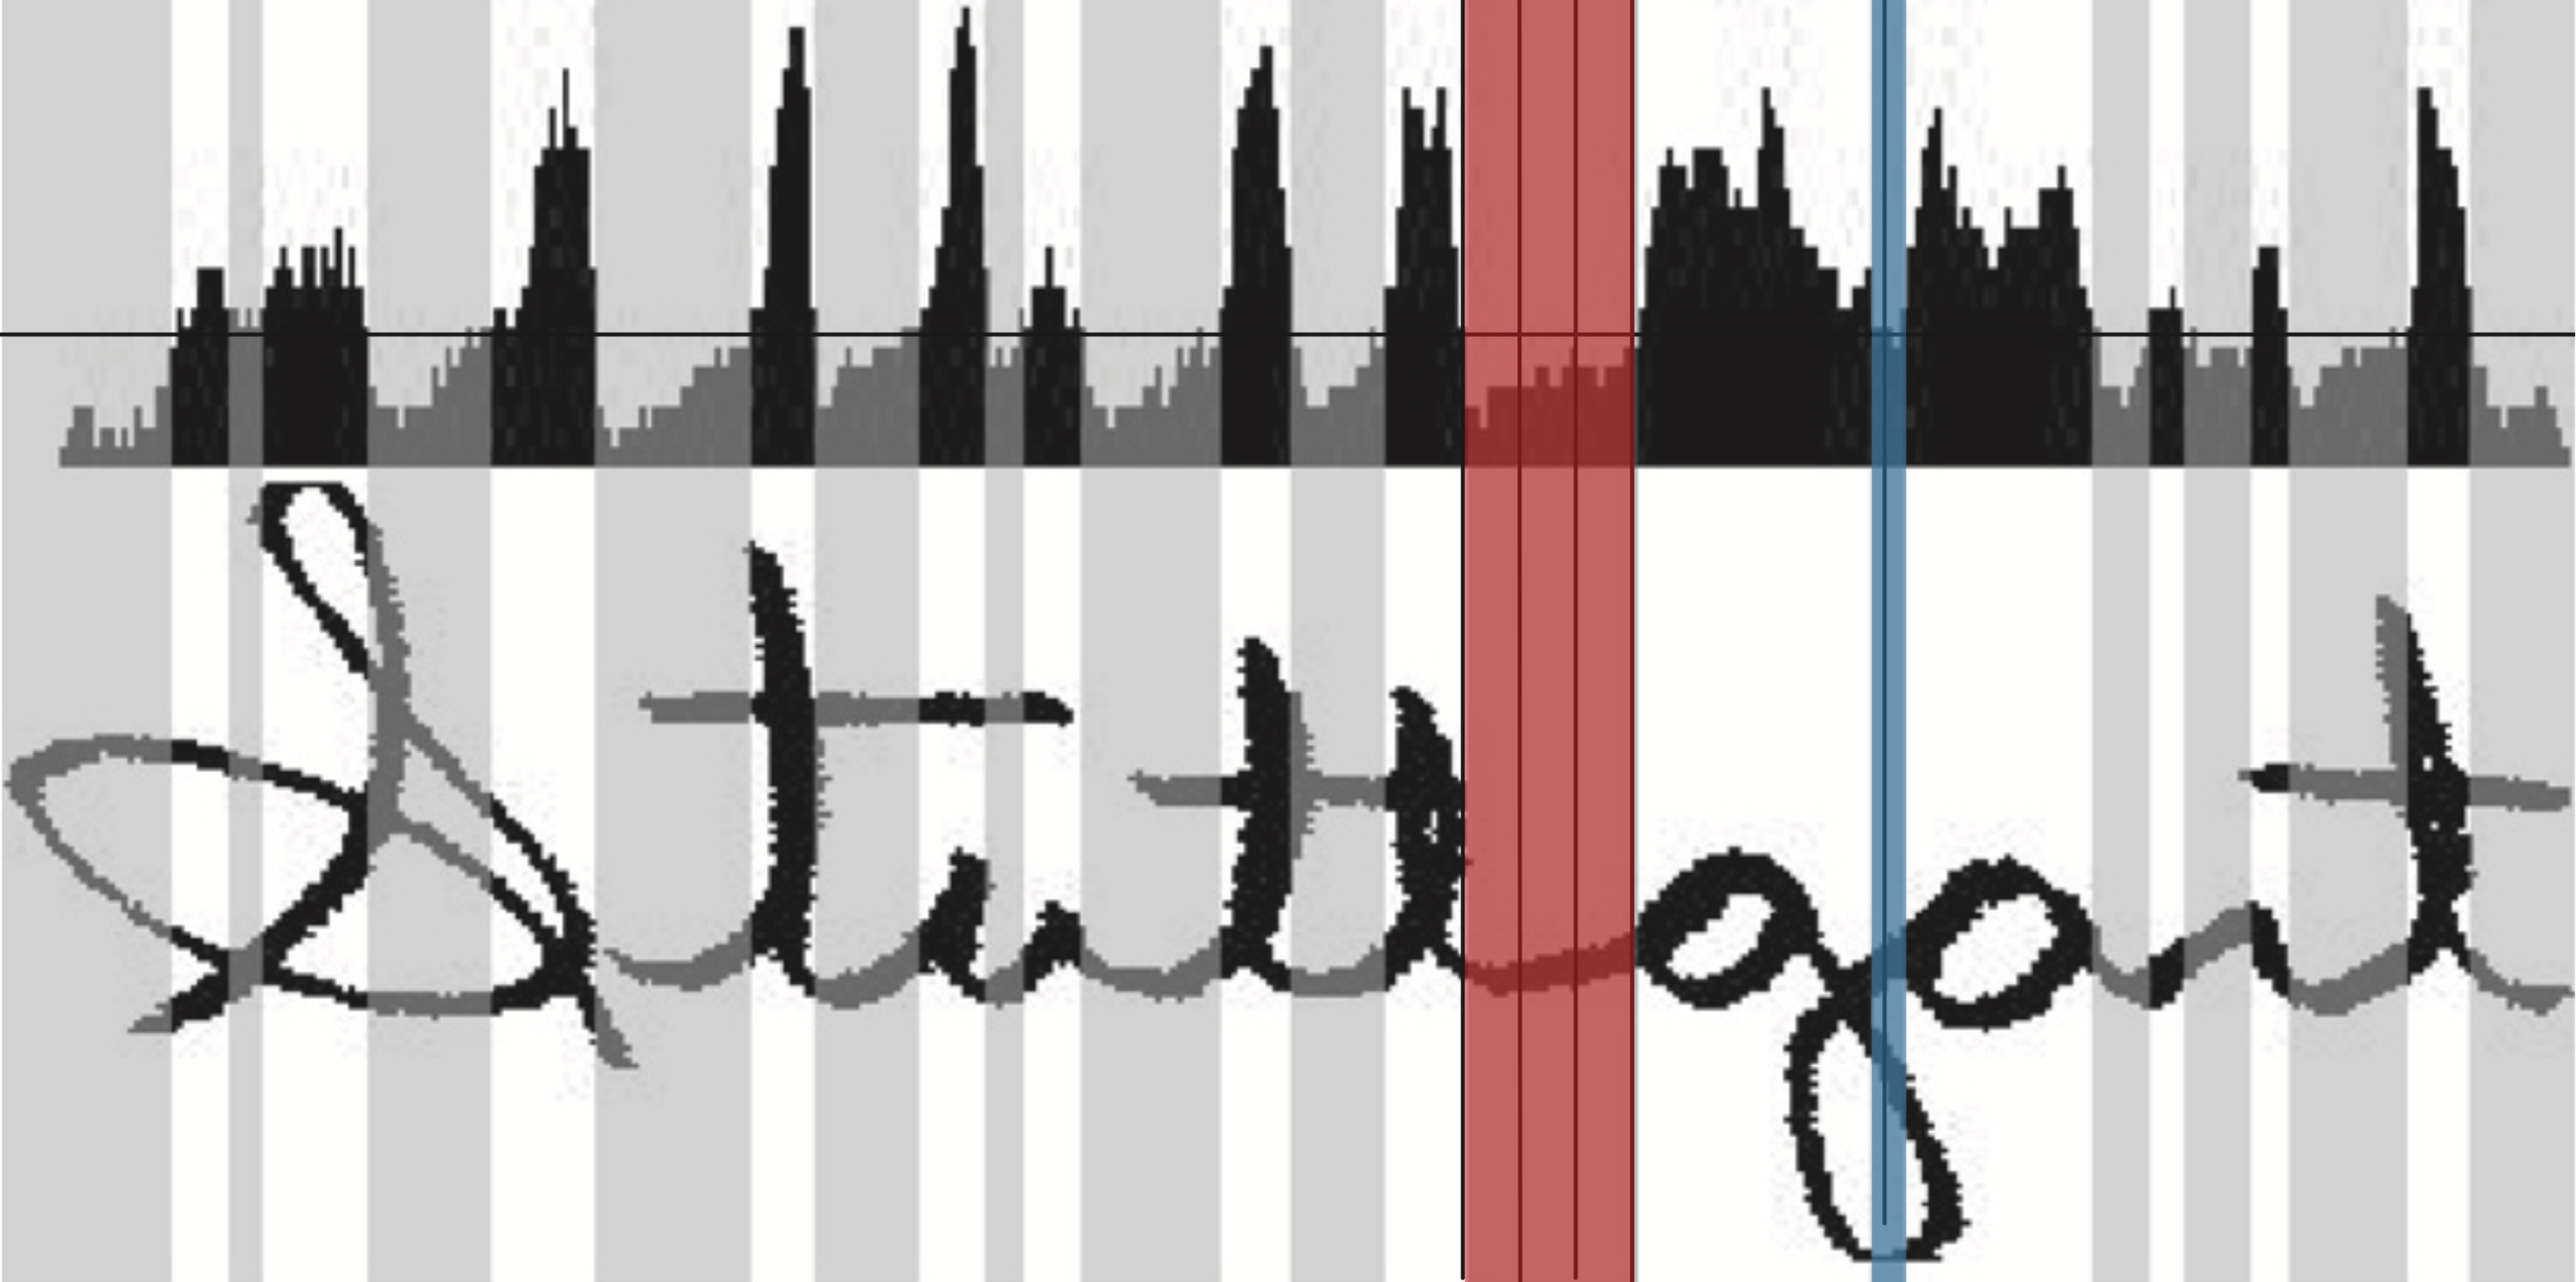
\includegraphics[width=\columnwidth]{shared/img/method/suspicious_regions.png}
		\caption{The vertical pixel density of the body of the image above the word image.  The threshold for suspicious regions is shown as a line in the histogram. The shaded areas show the suspicious regions. For the regions shaded in a color the lines associated with the segmentations points are drawn. The image is adapted from \cite{lee2012binary}.}
		\label{fig:method:segmentation:suspiciousRegions}
	\end{figure}

	Based on these regions the initial set of segmentation points is determined. If the width of a region is smaller than the minimum character width, the region results in one segmentation line in the middle of the regions, this case is illustrated by the blue region in \cref{fig:method:segmentation:suspiciousRegions}. In regions with a width that is equal to or greater than the minimum character width, the red region in \cref{fig:method:segmentation:suspiciousRegions}, segmentation points are placed at the end of the region and on intervals of the minimum character width that start at the beginning of the region. Before starting the segmentation these lines are filtered to ensure optimal placement. 

	Firstly all segmentation lines over a hole in the image are removed. This filtering is restricted to Latin alphabet, which as a number of letters with. It also assumes that it  does not occur that two letters are connected via a whole, although noise that was not removed could cause the occurrence of a hole between two letters. Holes are detected via region growing algorithm. 

	After all segmentation lines crossing a hole have been removed we move some of the segmentation lines in such a way that in the final image the distance between two segmentation lines is always greater than the minimum character width. This is done as follows: iterate over all pairs of lines that are present when you move from left to right through the image. If the distance between the lines that make up the pair is smaller than the the minimum character width remove the lines, and place a new line in the middle between those two lines. This process is then recursively repeated for the segmentation lines to the left of the new line and for the lines to the right of this line. 

	\timemachine{Show with an image.}

	The resulting set of segmentation points is used for the actual segmentation. 

\subsubsection{Select Sub-Image}
\label{sss:method:segmentaton:selectsubimage}
	As shown in \cref{alg:method:segmentation:algorithm} the algorithm keeps track of two lists, one with character images, \characters, and one with images that need to be segmented further, \segmentfurther. At the start of each iteration an image is selected for further segmentation for the second list. From this list the image with the highest width over height ratio is selected. This is done on the assumption that the widest image is the most likely to contain multiple characters. It should be noted that the height of the images is not the same for all images, as white borders are from \leftsubimage and \rightsubimage before they are stored in the either \characters or \segmentfurther. This reduces the influence of sloppy word bounding boxes on the segmentation.

\subsubsection{Select Segmentation Point}
\label{sss:method:segmentaton:selectssp}
	Given an image for further segmentation with multiple segmentation lines one needs to select along which segmentation line the image should be split. This is done based on two scores: the distance score and the vertical pixel density score. 

	The first promotes the selection of a segmentation line near the center of the image. This should avoid the chain failure problems. Let the $x$-coordinates of the segmentation line and the center of the image be represented by $l_x$ and $c_x$, respectively, the distance score is then defined as
		\begin{equation}\label{eq:method:segmenation:selectSP:distancecriterion}
			s_{\text{distance}} = \frac{\abs{c_x - l_x}}{c_x}.
		\end{equation}

	The second scores promotes the selection of segmentation points that indicate spaces where white space separates two characters. Let the height of the sub image be $w$ and $l_d$ the pixel density in the image underneath the line, the density score is then:
		\begin{equation}
			s_{\text{density}} = \frac{l_d}{w}.
		\end{equation}
	Both scores are summed, the line with the lowest score is selected as the segmentation point.

\subsubsection{Split}
\label{sss:method:segmentaton:splitimage}

	\begin{figure}
		\timemachine{Indicate $g$ and $s$ in the image.}
		\centering
		\subfloat[]{
			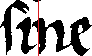
\includegraphics[width=6em, height=4em, keepaspectratio=True]{shared/img/method/split_straight_path.png}%
			\raisebox{1em}{\hspace{2em} $\to$ \hspace{2em}}
			
\includegraphics[width=6em, height=4em, keepaspectratio=True]{shared/img/method/split_straight_left.png}%
			\raisebox{1em}{\hspace{2em} $\&$ \hspace{2em}}
			
\includegraphics[width=6em, height=4em, keepaspectratio=True]{shared/img/method/split_straigt_right.png}%
			\label{fig:method:segmentation:splitting:straight}%
		}

		\subfloat[]{
			
\includegraphics[width=6em, height=4em, keepaspectratio=True]{shared/img/method/split_astar_path.png}%
			\raisebox{1em}{\hspace{2em} $\to$ \hspace{2em}}
			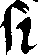
\includegraphics[width=6em, height=4em, keepaspectratio=True]{shared/img/method/split_astar_left.png}%
			\raisebox{1em}{\hspace{2em} $\&$ \hspace{2em}}
			
\includegraphics[width=6em, height=4em, keepaspectratio=True]{shared/img/method/split_astar_right.png}%
			\label{fig:method:segmentation:splitting:astar}%
		}
		\caption{Splitting based on a segmentation point, shown as a blue line, along \protect\subref{fig:method:segmentation:splitting:straight} a straight path and \protect\subref{fig:method:segmentation:splitting:astar} a path found with \astar. The used paths are shown in red. The original image is shown on the left of the arrow, the resulting sub images are shown on the right side of the arrow.}
		\label{fig:method:segmentation:splitting:comparison}
	\end{figure}

	The simplest way to split the image along the segmentation line, $l$, is to designate all pixel to the left of the line to \leftsubimage, and all pixels to the right of the line to \rightsubimage. However this can result in artifacts as illustrated in \cref{fig:method:segmentation:splitting:straight}, where part of the `n' is added to the `i', resulting in a letter that looks more like a `c' than an `i' in \leftsubimage.

	In \cref{fig:method:segmentation:splitting:astar} the image are split along a path that keeps both characters intact. This path is found by looking for a path from $s$ to $g$, the pixels on the segmentation line on the first and last row, respectively. From some pixel only its four-connected neighbors can be reached. The path is searched in an area with width minimum character width centered on the segmentation line, to restrict the path and computation time. The heuristic distance from pixel $n$ to the goal pixel, $g$:
	\begin{equation}\label{eq:method:segmentation:heuristic}
		h(n) = \abs{g_x - n_x} + \abs{g_y - n_y}.
	\end{equation}
	We chose the Manhattan distance as that best represents possible paths taken when walking along pixels in an image.

	The cost of getting from the start pixel, $s$, to pixel $n$ is defined as:
	\begin{equation}\label{eq:method:segmentation:costFunction}
		g(n) = 
		\begin{cases}
			g(n') + 1	& \text{if } n \text{ is a background pixel.}\\
			g(n') + i 	& \text{if } n \text{ is a foreground pixel on $l$.}\\
			\infty 		& \text{otherwise.}
		\end{cases}
	\end{equation}
	where $i$ is the intersection penalty and $n'$ is the four connected neighbor from which we reached $n$.

	\Cref{eq:method:segmentation:costFunction} allows the path along which the characters are separated to only intersect foreground pixels on the segmentation line. Furthermore the intersection penalty ensures that the characters are only split along a winding path if a straight path is not possible. We have set the intersection penalty, $i$, to 5. If there are no foreground pixels underneath the segmentation line, the distance function reduces to the Minkowski distance with $p = 1$. 

\subsubsection{Is Character}
\label{sss:method:segmentaton:segmentfurther}
\todo[inline]{How to determine if an image should be segmented further, or if it is an character.}

\subsubsection{Continue}
\label{sss:method:segmentaton:termination}
\todo[inline]{Wanneer stoppen we met ons lusje}